\documentclass[12pt,a4wide]{article}
\usepackage{verbatim}
\usepackage{listings}
\usepackage{graphicx}
\usepackage{a4wide}
\usepackage{color}
\usepackage{amsmath}
\usepackage{amssymb}
\usepackage[dvips]{epsfig}
\usepackage[T1]{fontenc}
\usepackage{cite} % [2,3,4] --> [2--4]
\usepackage{shadow}
\usepackage{hyperref}
\usepackage{fancyhdr}
\pagestyle{fancy}

\setcounter{tocdepth}{2}

\lstset{language=c++}
\lstset{basicstyle=\small}
\lstset{backgroundcolor=\color{white}}
\lstset{frame=single}
\lstset{stringstyle=\ttfamily}
\lstset{keywordstyle=\color{red}\bfseries}
\lstset{commentstyle=\itshape\color{blue}}
\lstset{showspaces=false}
\lstset{showstringspaces=false}
\lstset{showtabs=false}
\lstset{breaklines}
\begin{document}
\fancyhead[CO,CE]{Lars Christian Hauge}
\fancyhead[RO,RE]{15.09.13}
\section*{Project 1}

\section*{Abstract}
In this project we solved a differential equation by manipulating it into a tridiagonal matrix and we developed our own tridiagonal solver that proved much more efficient for this problem than Armadillo's LUdecompostion.
Lastly we discovered it was more effective to multiply matrices row-wise than column-wise. 

\section*{Introduction}
The main task for this project is to solve the differential equation
\[
-u''(x) = f(x), \hspace{0.5cm} x\in(0,1), \hspace{0.5cm} u(0) = u(1) = 0
\]
where $f(x) = 100e^{-10x}$. We are going to solve this numerically and the derivative we are going to approximate by
\[
   -\frac{v_{i+1}+v_{i-1}-2v_i}{h^2} = f_i  \hspace{0.5cm} \mathrm{for} \hspace{0.1cm} i=1,\dots, n.
\]
Our first task is to transform this into a matrix, and then come up with an algorithm that will solve this
problem. We also have to compare the error we get for different step lengths h, e.g. the number of points we use.
All of this we have to implement into c++, a language I have never used before. 
We are then going to implement the LUdecomposition method to compare it to our own algorithm.
The way we are going to compare it is by measuring the time taken for the programs to run. 

\section*{Methods}
The first thing we have to show is that 
   $-\frac{v_{i+1}+v_{i-1}-2v_i}{h^2} = f_i \hspace{0.1cm} \mathrm{for} \hspace{0.1cm} i=1,\dots, n$
can be written on the form
\[
   {\bf A}{\bf v} = \tilde{{\bf b}},
\]
where
\begin{equation}
    {\bf A} = \left(\begin{array}{cccccc}
                           2& -1& 0 &\dots   & \dots &0 \\
                           -1 & 2 & -1 &0 &\dots &\dots \\
                           0&-1 &2 & -1 & 0 & \dots \\
                           & \dots   & \dots &\dots   &\dots & \dots \\
                           0&\dots   &  &-1 &2& -1 \\
                           0&\dots    &  & 0  &-1 & 2 \\
                      \end{array} \right),
	      \hspace{0.5cm}             	\tilde{{b_i}} = {h^2}{f_i}.
\end{equation}
The first thing we realise is that  $-\frac{v_{i+1}+v_{i-1}-2v_i}{h^2} = f_i$ can be written as a set of linear equations.
\[
-{v_{1}}+2{v_{0}} = \tilde{b_{0}} 
\]
\[
-{v_2} + 2{v_1} - {v_0} = \tilde{b_1} 
\]
\[
-{v_2} + 2{v_1} - {v_0} = \tilde{b_2} 
\]
\[
\dots = .
\]
\[
\dots = .
\]
\[
-{v_{n+1}} + 2{v_n} - {v_{n-1}} = \tilde{b_n}
\]
This we can again write as 
\begin{equation}
{v_1}
	\left(\begin{array}{c}
                           2\\
                           -1\\
                           \dots \\
                          \dots  \\
                          \dots \\
                           0\\
                      \end{array} \right) +
{v_2} 
\left(\begin{array}{c}
-1\\
2\\
-1\\
\dots \\
\dots \\
0\\
\end{array} \right) + 
{v_3}
\left(\begin{array}{c}
0\\
-1\\
2\\
-1\\
\dots \\
0\\
\end{array} \right) + \dots +
{v_{n-1}}
\left(\begin{array}{c}
0\\
0\\
\dots\\
-1 \\
2 \\
-1\\
\end{array} \right) +
{v_n}
\left(\begin{array}{c}
0\\
0\\
\dots\\
\dots \\
-1 \\
2\\
\end{array} \right) = 
\left(\begin{array}{c}
\tilde{b_1}\\
\tilde{b_2}\\
\dots\\
\dots \\
\dots \\
\tilde{b_n}\\
\end{array} \right)
\end{equation}
Which can be written as
\[
  \left(\begin{array}{cccccc}
                           2& -1& 0 &\dots   & \dots &0 \\
                           -1 & 2 & -1 &0 &\dots &\dots \\
                           0&-1 &2 & -1 & 0 & \dots \\
                           & \dots   & \dots &\dots   &\dots & \dots \\
                           0&\dots   &  &-1 &2& -1 \\
                           0&\dots    &  & 0  &-1 & 2 \\
                      \end{array} \right)
\left(\begin{array}{c}
{v_1}\\
{v_2}\\
\dots \\
\dots \\ 
\dots \\
{v_n} \\
\end{array} \right) = 
\left(\begin{array}{c}
\tilde{b_1}\\
\tilde{b_2}\\
\dots \\
\dots \\ 
\dots \\
\tilde{b_n} \\
\end{array} \right)
\]

Our next task is to come up with an algorithm that could solve this problem. We already heard in the lectures that all that is needed for this problem
is a subtraction and a forward substitution and then a backwards substitution. The way I did this was to 
remove the first non-zero element on each line by subtracting the line with the line above it. With that approach we get an upper
triangular matrix where we can easily find the solution. We have the last element of the solution in the last row,
so we can just work our way backwards. 

I then implemented this into c++ and got this program:
\lstinputlisting{project1.cpp} %% Remember to remove the bottom of the file

For plotting the results for various step lengths I wrote it to file and used python to plot.
\lstinputlisting{project1plot.py}

I calculated the maximum error for different values of n, as instructed in the exercise text. How I did it is included in the main program.

Then it is on to the LU-decomposition, we shall solve the exact same equation as before just now it is another method involved. 
To solve this we use the c++ package armadillo and its built in function LU that splits a matrix into an upper triangular and a lower triangular matrix.
With this we are quipped to solve the entire equation and we only need to use the built-in armadillo function solve(). We see
that the LU-decomposition gives the exact same results as the tridiagonal solver from earlier.
\lstinputlisting{LUdecomp.cpp} 
Our task however is to measure the difference in time and this I did by the built-in Unix command "time" before running the program.
The last task asked us to multiply two matrices, row-wise and column-wise, to see which is the most effective. I again use armadillo to create
two matrices of equal size with random elements, and then use the code presented in the text to multiply them. I used the built-in "time" function in Unix to measure the time the programs use.
The program for multiplying row-wise:
\lstinputlisting{row.cpp}
and column-wise:
\lstinputlisting{column.cpp} 

\section*{Results}
The first thing we are asked to say something about is the number of flops in our algorithm. In my algorithm I get
${8}{n}$ flops, if I use the fact some of the elements can only have the values -1 and 2 I could probably get it down some more,
but that will not solve a general tridiagonal matrix equation. It is either way much better than the LU-decomposition that uses
$\frac{2}{3} {n^3}$ flops. Standard Gaussian elimination takes $\frac{2}{3} {n^3}$ flops, so that would be even more ineffective.

From our tridiagonal solver and the LU decomposition we got some plots, unfortunately I could not get plots for n = 10000 for LU decomposition.
We see from the plots that both methods give about the same result, and that for small n they are not that accurate. We have to use almost 1000 points before
we get acceptable results. The results for the tridiagonal solver for n = 10000 and 100000 are almost perfect and they do not take that long time to produce, 
while for LU you use a lot of time for the same results. Figure~\ref{n10} shows us n = 10,  figure~\ref{n100} n = 100, figure~\ref{n1000} n = 1000 and figure~\ref{n10000} shows us the tridiagonal solution for n = 10000 and 100000.
\begin{figure}
	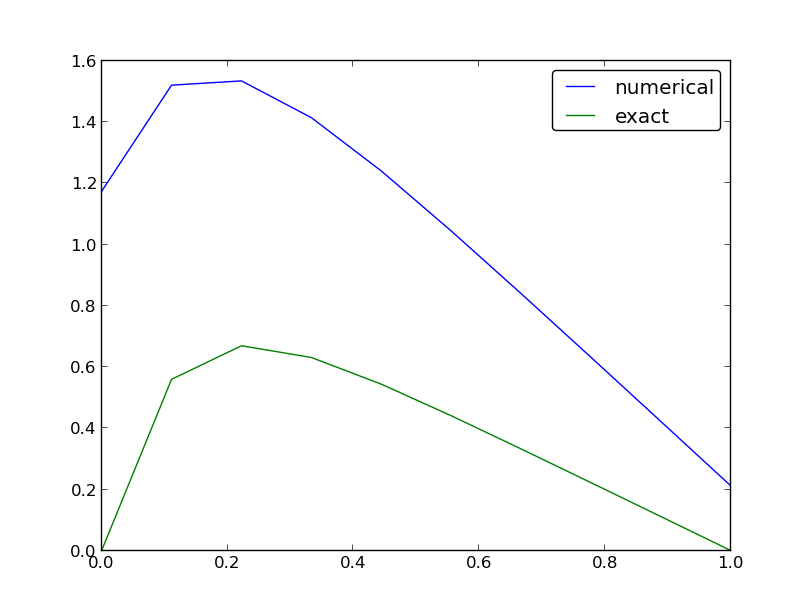
\includegraphics[width=8cm]{project1n10}
	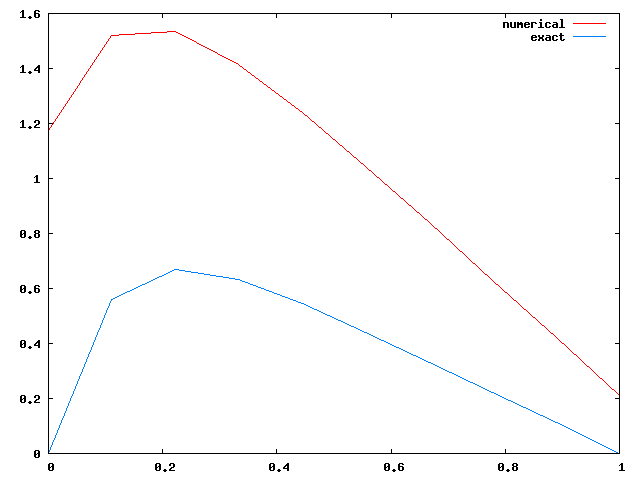
\includegraphics[width=8cm]{LUn10}
	\caption{Tridiagonal solver to the left, LU decompostion to the right for n=10}
	\label{n10}
\end{figure}
\begin{figure}
	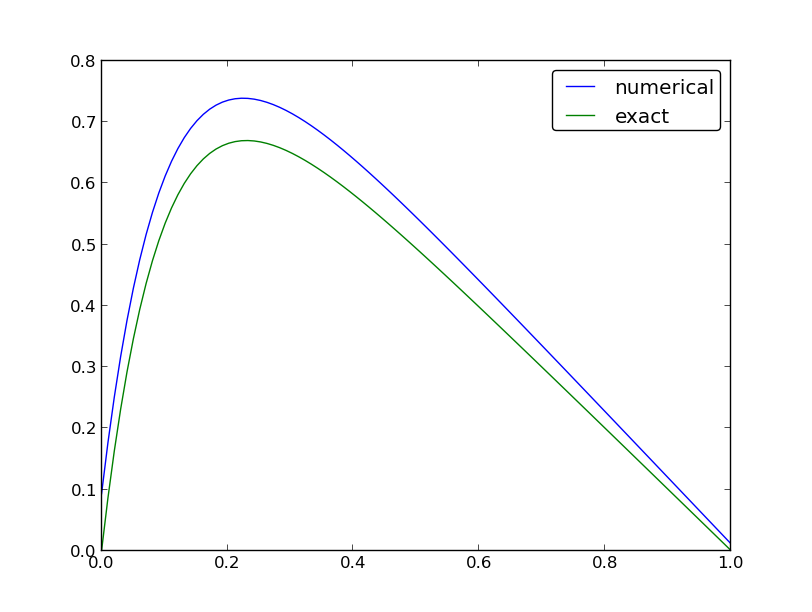
\includegraphics[width=8cm]{project1n100}
	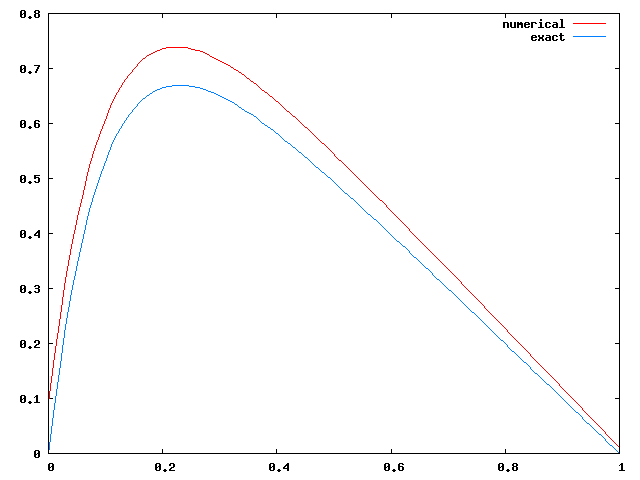
\includegraphics[width=8cm]{LUn100}
	\caption{Tridiagonal solver to the left, LU decompostion to the right for n=100}
	\label{n100}
\end{figure}
\begin{figure}
	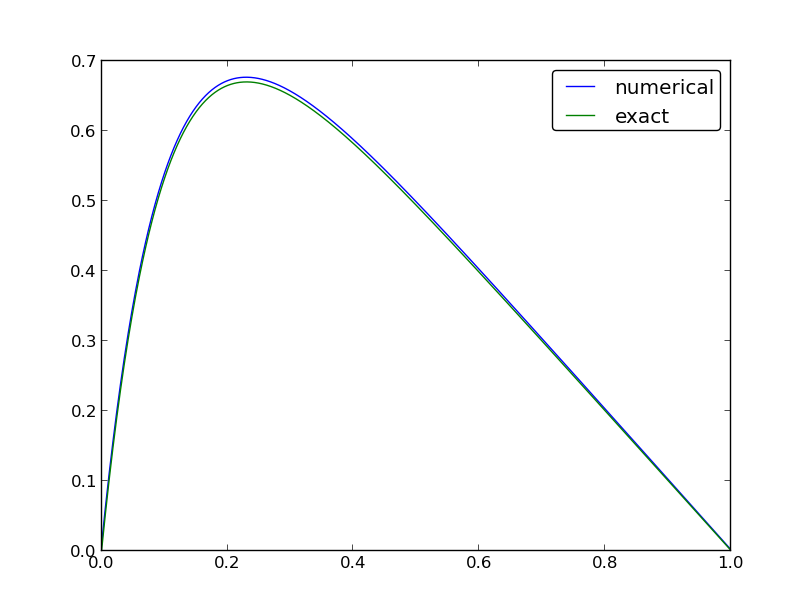
\includegraphics[width=8cm]{project1n1000}
	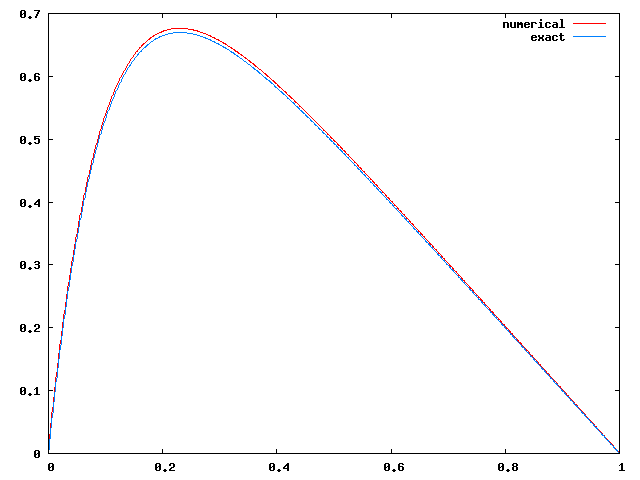
\includegraphics[width=8cm]{LUn1000}
	\caption{Tridiagonal solver to the left, LU decompostion to the right for n=1000}
	\label{n1000}
\end{figure}
\begin{figure}
	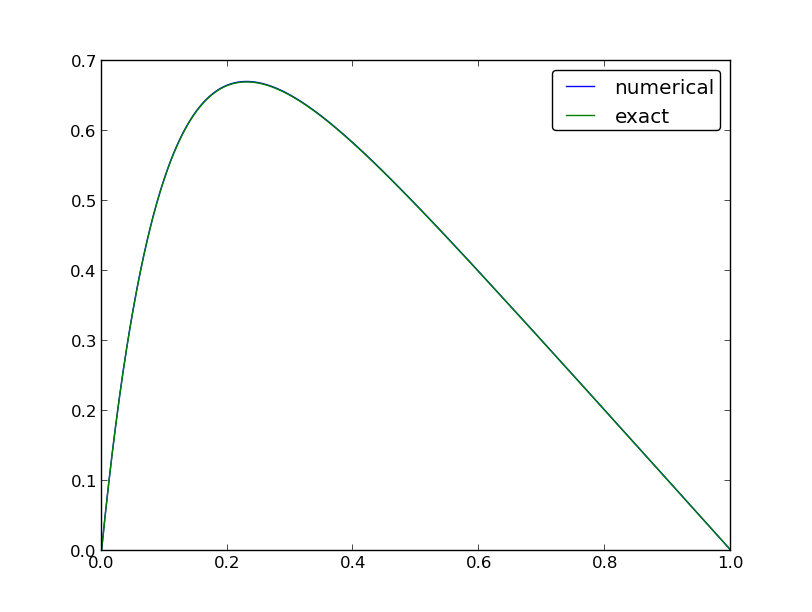
\includegraphics[width=8cm]{project1n10000}
	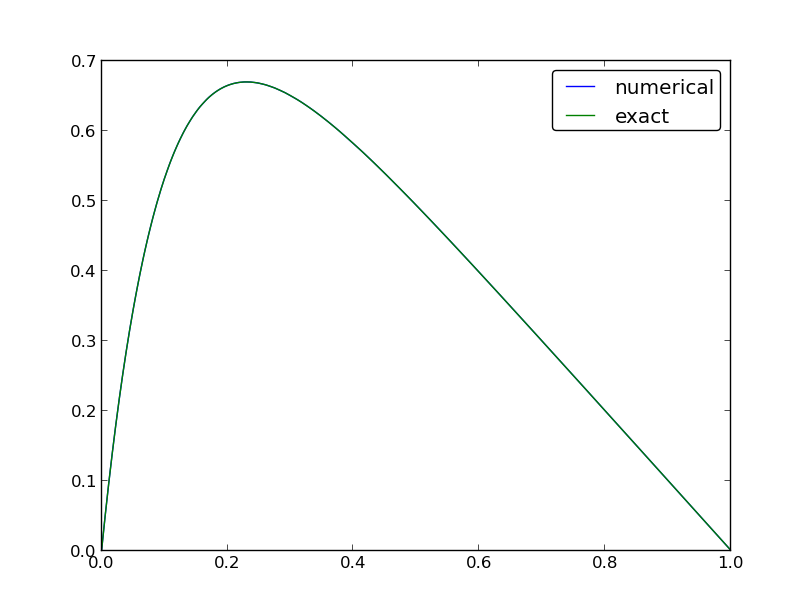
\includegraphics[width=8cm]{project1n100000}
	\caption{To the left tridiagonal solver for n = 10000, right for n = 100000}
	\label{n10000}
\end{figure}

I have also computed the maximum relative error for each n for the tridiagonal solver and plotted them with respect to ${log_{10}}({h})$ and ${log_{10}}({n})$.
The relavtive error in a table:
\begin{tabular}{|c|c|}
\hline
${log_{10}}({n})$ & $\epsilon$ \\ \hline
	1 & 1.76259 \\ \hline
	2 & 0.348336 \\ \hline
	3 & 0.30541 \\ \hline
	4 & 0.301465 \\ \hline
	5 & 0.301073 \\ \hline
	\hline
\end{tabular} 
Figure~\ref{error}shows the relative error as a plot for different n values and h values. We say they are almost the exact inverse of each other. 
The error falls steeply from n = 10 to 100, but after that it seeks towards 0.3.

\begin{figure}
	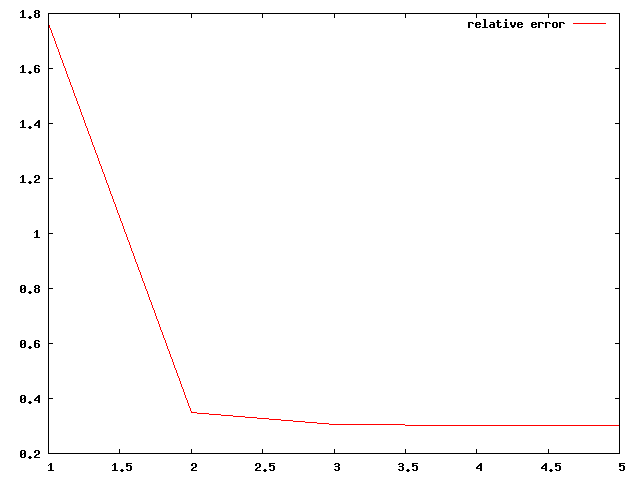
\includegraphics[width=7cm]{relativeerror}
	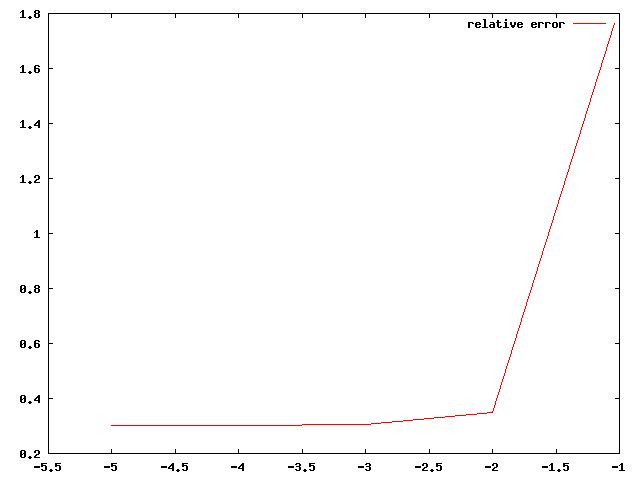
\includegraphics[width=7cm]{relativeerror1}
	\caption{Relative error for different n values for the left plot, the right plot is for different h values}
	\label{error}
\end{figure}


Time usage of the different solvers I have said much about and here comes some numbers on the time usage for different n for the two numerical methods.
We see what I have said earlier that the tridiagonal solver is extremely efficient for this problem, while the otherwise efficient LU decomposition 
provides the same results after a much longer time. 
\begin{tabular}{|c|c|c|}
	\hline
	${log_{10}}({n})$ & time tridia & time LU dec \\ \hline
	1 & 0.015s & 0.018s \\ \hline
	2 & 0.013s & 0.019s \\ \hline
	3 & 0.014s & 0.365s \\ \hline
	4 & 0.215s & 4min30.182s \\ \hline
	5 & 0.254s & armadillo hates me \\ \hline
	\hline
\end{tabular}
We also have that last exercise to consider where we shall see what is the most efficient of row and column multiplication of matrices. 
We are asked to consider the case ${10^4}\times{10^4}$, that would take many hours for each of the multiplications, and I soon gave that up.
The results I got in the end was:
\begin{tabular}{|c|c|c|}
	\hline
	${log_{10}}({n})$ & row & column \\ \hline
	1 & 0.002s & 0.002s \\ \hline
	2 & 0.027s & 0.029s \\ \hline
	3 & 27.467s & 30.902s \\ \hline
	\hline
\end{tabular}
	
We see that row multiplication goes slightly faster than column multiplication. For ${10^4}$ the time difference will probably grow to a few hours , which is significant.

\section*{Conclusion}
We have seen how easily one can solve differential equations numerically if you know the right methods, and the correct step length for the precision you want. It was not 
very much difference in time even if you used a step length $\frac{1}{10}$ of what you need if you use the correct method. 

In this project we have discovered that a simple problem can be solved considerably faster by just using a different algorithm, and that seemingly equal things
like row multiplication and column multiplication, take a different amount of time. We also have a basis for future problems where we need to equations with a tridiagonal matrix. 
It was also a nice first experience with c++ and latex, the exercise gave me great experience for future work with those. 




\end{document}